\documentclass{article}
\usepackage[utf8]{inputenc}
\usepackage[english]{babel}
\usepackage{amssymb}
\usepackage{amsmath}
\usepackage{graphicx}
\usepackage{enumerate}

\usepackage{geometry}
\geometry{left=2.5cm,right=2.5cm,top=2cm,bottom=2cm}

\setlength{\parskip}{0.5em}
\setlength{\parindent}{0em}
\renewcommand{\baselinestretch}{1.0}

\title{Assignment 2}
\author{COL 352\\
    Introduction to Automata \& 
    Theory of Computation}
\date{}

\begin{document}
    \maketitle
    
    \section*{Problem 1} Design DFA for the following languages over $\{0, 1\}$
    \begin{enumerate}[(a)]
        \item The set of all strings such that every block of of five consecutive symbols have at least two 0’s
        \item The set of strings with an equal number of 0’s and 1’s such that each prefix has at most one more 0 than
1’s and at most one more 1 than 0’s
    \end{enumerate}
    
    \textbf{Solution} : 
    
    (a)
    
    (b) If there is no explanation of the states/DFA, at most 5/10 will be given.
    \begin{center}
        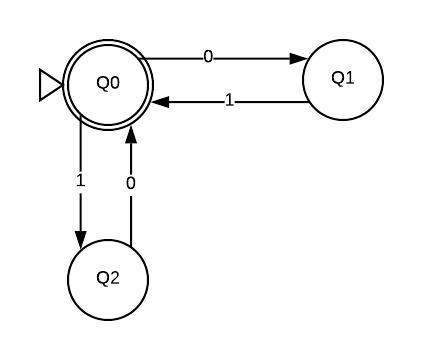
\includegraphics[width=0.5\textwidth]{Images/a2-q1-2.jpeg}
    \end{center}
    
    
    
    \section*{Problem 2} Design NFA for the following languages
    \begin{enumerate}[(a)]
        \item The set of strings over ${a, b}$ that have the same value when multiplied from left to right as from left to right. The rules of multiplication are $a \times a = b$, $b \times b = a$, $a \times b = b$, $b \times a = b$. Note that $((a \times b) \times b) = a$ and $(a \times (b \times b)) = b$, i.e. it is not associative
        \item The set of strings of the form $\{xwx^R ~|~ x, w$ are strings over 0,1 of non-zero length\}
    \end{enumerate}
    
    \textbf{Solution} : 
    
    
    \section*{Problem 3} Prove or disprove $(r+s)^* = r^* + s^*$, where $r$, $s$ and $t$ are regular expressions and $r=s$ implies $L(r)=L(s)$)
    
    \textbf{Solution} :
    
    Let $\Sigma = \{0, 1 \}$ and $r = 0^*$, $s = 1^*$
    
    Then, $(r + s)^* = \epsilon \cup \{ 0, 1 \} \cup \{ 0, 1 \}^2 \cup \dots$
    and, $r^* + s^* = \epsilon \cup \{ 0\} \cup \{ 0 \}^2 \cup \dots \cup \{ 1\} \cup \{ 1 \}^2 \cup \dots$
    
    Now, consider a string $01$.
    
    Clearly, $01 \in \{0, 1 \}^2 \Rightarrow 01 \in (r + s)^*$, but $01 \notin r^* + s^*$
 
    Hence, $(r+s)^* \neq  r^* + s^*$
    
    
    \section*{Problem 4} Which of the following are regular sets
    \begin{enumerate}[(a)]
        \item $\{ 0^{2^n} |~ n \geq 1\}$
        \item $\{ xx^Rw |~ x, w \in (0 + 1)^+ \}$
    \end{enumerate}
    
    \textbf{Solution} : 

    (a) Let $L$ denote the set, then assuming that it is regular, let $n \geq 1$ denote the pumping lemma constant

    \quad Consider the string $0^{2^n} \in L = 0^{p}0^{q}0^{r}$ with $p + q + r \geq n$, $q \geq 1$ and $p + q \leq n$. 
    
    \quad Now, from pumping lemma, $\forall i \geq 0,0 ^{p}0^{iq}0^{r} \in L$, i.e. $p + iq + r = 2^m$, for some $m \geq 1$. 
    
    \quad Setting $i = 2$, gives $p + 2q + r = 2^m$, and since $p + q + r = 2^n \Rightarrow 2^n + q = 2^m$, i.e. $q$ is a power of 2. 
    
    \quad Specifically, since $n, m$ are integers and $q \geq 1, q = 2^n$.
    
    \quad But this means that $q > n$, since $n \geq 1$
    and so, $p + q > n$  - a contradiction. Thus the $L$ is not a regular set.
    
    (b) Let $L$ denote the set, then assuming that it is regular, let $n \geq 1$ denote the pumping lemma constant
    
    \quad Consider the string $0^n1.10^n.1 \in L = 0^{l}0^{m}0^{n - m - l}1.10^n.1, ~1 \leq m < n, ~0 < l < n$, with $x = 0^l, ~ y = 0^{m}$
    
    \quad Now, from pumping lemma, $\forall i \geq 0, ~xy^iz \in L$, as $|xy| \leq n$ and $y \geq 1$

     \quad Setting $i = 2$, gives $xy^2z = 0^{n + m}1.10^n.1 \in L$ 
     
     \quad But since $n + m > n$, so $xy^2z \notin L$ - a contradiction. Thus the $L$ is not a regular set.  
     
    Also accepted : Solutions that use the Myhill-Nerode theorem correctly


    \section*{Problem 5} Is the set $\frac{1}{2}(L) = \{ x|~ \exists y$ such that $|x| = |y|, ~xy \in L \}$
    
    \textbf{Solution} : Since, $L$ is a regular language, so, let, $M = (Q,\Sigma, \delta, q_0, F)$ be the DFA that accepts $L$.
    
    Let $L' = \frac{1}{2}L $. We will construct a DFA $M' = (Q',\Sigma, \delta', q_0', F')$ which accepts $L'$ and hence prove that it is a regular language.
    \begin{itemize}
        \item $Q' = Q \times 2^Q $
        \item Let $S\in2^Q$. Define 
         $prev(S)= \{q \in Q\ | \ \exists\ a \in \Sigma,\ q' \in S\ s.t.\ \delta(q,a) = q'\}$
        \item $\delta'((q,S), a) = (\delta(q,a),prev(S))$
        \item $q_0' = (q_0,F)$
        \item $F' = \{(q,S), q\in S\}$
    \end{itemize}
    
    $F_1 = prev(F)$ will give us all the states in $M$ from where we can reach a final state of $M$ on reading a string of length 1. Similarly, $F_n = prev(F_{n-1})$ will give us all the states in $M$ from where we can reach a final state of $M$ on reading a string of length n.
    
    \begin{itemize}
        \item Let, $xy \in L$ and $|x| = |y| = n$. $M$ reaches to a state $p$ after reading $x$ and from $p$ it reaches a final state $f$ on reading $y$. So, $p \in F_n$. And, on reading $x$, $M'$ will reach a state $(p, F_n)$. By definition of $F'$, it is a final state of $M'$. So, $xy$ will be accepted by $M'$.
        \item Now, let $x$ be accepted by $M'$ and $|x| = n$. So, let, $M'$ reaches a state $(p, P)$ where $p \in P$ on reading $x$. Also, $P = F_n$. So, there exists a string $y$, reading which we can reach from $p$ to a final state in $M$. So, $xy$ is accepted by $M$.
    \end{itemize}
    Hence, $L'$ is the language accepted by $M'$.
    

    Regarding the grading:
    \begin{itemize}
        \item If you have simply specified the DFA with no explanation, you will get at most 5/10.
        \item You need to prove that any string in $\frac{L}{2}$ will be accepted by the DFA \textbf{AND} any string accepted by the DFA will be contained in $\frac{L}{2}$. 
    \end{itemize}
    
\end{document}
